\chapter{Dispersión $e^{-}e^{+}\longrightarrow \mu^{+}\mu^{-}$}


Author: David Andrés Noreña Blandón

El proceso tratado es la dispersión inelástica de un par electrón positrón. A partir de este proceso, se generan 
un par partícula-antipartícula correspondiente a muón-antimuón, en este documento se calcula la sección eficaz de la producción
muón-antimuón. Los campos fermiónicos son: del electrón $\psi_e$, del positrón es $\bar{\psi}_e$, del muón $\psi_{\mu}$ y del antimuón $\bar{\psi}_{\mu}$ \\
La masa del par inicial no se considera debido a que la energía involucrada es mucho mayor que la masa del electrón. La masa del 
 muón y el antimuón es $m_{\mu}$ cuyos cuadrimomentos son $p_{-}, p_{+}$ respectivamente. Los cuadrimomentos del electrón y del positrón son $k_{-}, k_{+}$, 
Este proceso se puede denotar por :
\[
e^{-}(k_{-})e^{+}(k_{+})\longrightarrow \mu^{+}(p_{+})\mu^{-}(p_{-}) 
\]

El objetivo es calcular los elementos de la matriz $S$ y la amplitud de decaimiento $\Gamma$ para este proceso.
En la figura 1 se muestra un diagrama de Feynman del proceso en estudio.

\section{Lagrangiano}
El término relevante del lagrangiano del modelo estándar es:
\begin{equation}
 \mathcal{L}=\bar{e}_L\gamma^{\nu}e_L A_{\nu}\bar{\mu}_L\gamma^{\mu}\mu_L A_{\mu}
\end{equation}

\section{Matriz S}
\begin{figure}
\begin{center}
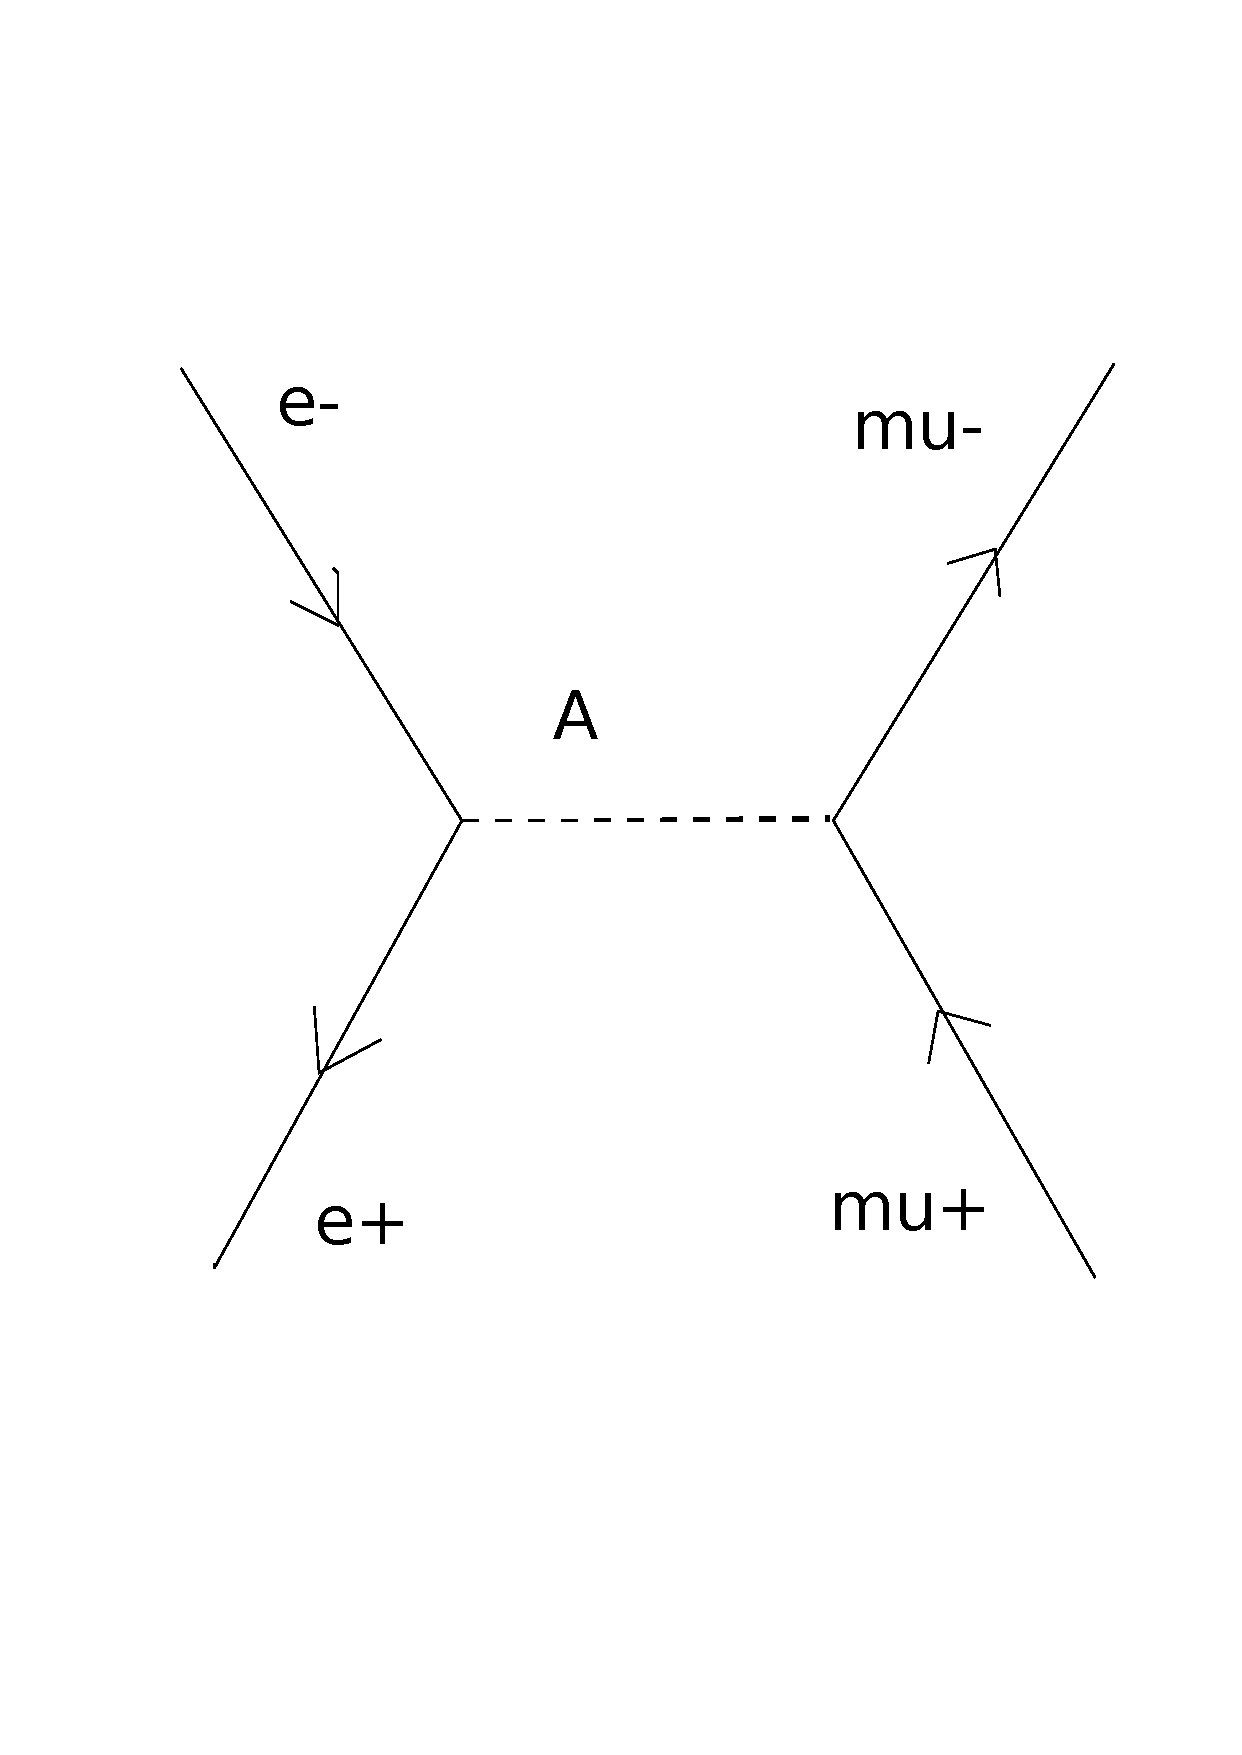
\includegraphics[width=0.5\textwidth]{./ProcesoDavid.pdf}
 % Proceso_David.pdf: 0x0 pixel, 0dpi, 0.00x0.00 cm, bb=
 \caption{Diagrama de Feynman del proceso}
\end{center}
\end{figure}
El Hamiltoniano de interaccion deriva del lagrangiano de la manera usual. Para la dispersión de este caso

\begin{equation}
  \mathcal{H}_I=-:\mathcal{L}:
=-:\bar{\psi}\gamma^{\mu}\psi\phi:
\end{equation}
Ahora miremos el segundo término en la expansión de la matriz $S$
\[
 S^{(2)}=\frac{(-i)^2}{2!}\int \int d^4x_1 d^4x_2 T\{\mathcal{H}_I(x_1)\mathcal{H}_I(x_2)\}
\]
\[
 = \frac{(-i)^2}{2!}\int \int d^4x_1 d^4x_2 T\{:(\bar{\psi}_e\gamma^{\mu}\psi_e\phi)_{x_1}(\bar{\psi}_{\mu}\gamma^{\mu}\psi_{\mu}\phi)_{x_2}:\}
\]

Donde el único término que contribuye al elemento de matriz en el proceso viene dado por:
\[
 S^{(2)}=\frac{(-i)^2}{2!} \int \int d^4x_1 d^4x_2 \phi(x_1)\phi(x_2):(\bar{\psi}_e\gamma^{\mu}\psi_e)_{x_1}(\bar{\psi}_{\mu}\gamma^{\mu}\psi_{\mu})_{x_2}:
\]
Con 
\[
 \phi(x_1)\phi(x_2)=i\Delta_F (x_1-x_2)
\]
Y además:
\[
:(\bar{\psi}_e\gamma^{\mu}\psi_e)_{x_1}(\bar{\psi}_{\mu}\gamma^{\mu}\psi_{\mu})_{x_2}:=:\bar{\psi}_e(x_1)\gamma^{\mu}\psi_e(x_1)\bar{\psi}_{\mu}(x_2)\gamma^{\mu}\psi_{\mu}(x_2):
\]
Descomponiendo los campos fermiónicos en $\psi_+$ y $\psi_-$, el término que contribuye es:
\[
 -\phi(x_1)\phi(x_2)\bar{\psi}^{\alpha}_{e+}(x_1)\gamma^{\mu}\bar{\psi}^{\beta}_{\mu-}(x_2)\psi^{\alpha}_{e+}(x_1)\gamma^{\mu}\psi^{\beta}_{\mu-}(x_2)
\]
  

El elemento de la matriz $S$ entre el estado inicial y el estado final es, simplificando la notación
\[
 S^{(2)}_{fi}=\frac{(-i)^2}{2!} \int \int d^4x_1 d^4x_2 i\Delta_F (x_1-x_2)
\]
\[
\times \langle \mu^{-}(\mathbf{p}_{-})\mu^{+}(\mathbf{p}_{+})|\bar{\psi}^{\mu}_{-}(x_2)\gamma^{\nu}{\psi}^{\mu}_{-}(x_2)\bar{\psi}^{e}_{+}(x_1)\gamma^{\mu}\psi^{e}_{+}(x_1)|e^{+}(\mathbf{k}_{+})e^{-}(\mathbf{k}_{-}) \rangle
\]
El estado de Fock de dos partículas es: 
\begin{equation}
 |e^{+}(\mathbf{k}_{+})e^{-}(\mathbf{k}_{-})\rangle=\sqrt{\frac{1}{V}}b_{k_{-}}^{\dagger}d_{k_{+}}^{\dagger}|0\rangle
\end{equation}
\begin{equation}
 |\mu^{+}(\mathbf{p}_{+})\mu^{-}(\mathbf{p}_{-})\rangle=\sqrt{\frac{1}{V}}B_{p_{-}}^{\dagger}D_{p_{+}}^{\dagger}|0\rangle
\end{equation}
Donde $b$ y $d$ son los operadores creación y aniquilación para el electrón, $B$ y $D$ son los operadores creación y aniquilación
del muón.\\
Usando la descomposición de Fourier de los campos fermiónicos, se calcula la acción de los operadores de campo sobre los estados
de las partículas, dando como resultado:
\[
 \bar{\psi}^{e}_{+}(x_1)\gamma^{\mu}\psi^{e}_{+}(x_1)|e^{+}(\mathbf{k}_{+})e^{-}(\mathbf{k}_{-}) \rangle=
\]
\[
\frac{1}{(2\pi)^3\sqrt{2E_{k_{+}} V}}\frac{1}{(2\pi)^3\sqrt{2E_{k_{-}} V}}\bar{v}(\mathbf{k_{+}})\gamma^{\mu}\bar{u}(\mathbf{k_{-}})e^{-i(k_{+}+k_{-}).x_1}|0\rangle
\]
\[
\langle \mu^{-}(\mathbf{p}_{-})\mu^{+}(\mathbf{p}_{+})|\bar{\psi}^{\mu}_{-}(x_2)\gamma^{\nu}{\psi}^{\mu}_{-}(x_2)
\]
\[
=\langle 0|\frac{1}{(2\pi)^3\sqrt{2E_{p_{+}} V}}\frac{1}{(2\pi)^3\sqrt{2E_{p_{-}} V}}\bar{u}(\mathbf{p_{+}})\gamma^{\nu}{u}(\mathbf{p_{-}})e^{i(p_{+}+p_{-}).x_2}
\]
Luego de integrar, tomando en cuanta la conservación de la carga, el elemento de matriz es: 

Así nos queda que el elemento de matriz de primer orden entre los estados inicial y final es:
\[
 S^{(2)}_{fi}=-e^2 \int \int d^4x_1d^4x_2 e^{i(p_{+}+p_{-}).x_2-i(k_{+}+k_{-}).x_1}
\]
\[
\times \frac{[\bar{u}(\mathbf{p_-})\gamma^{\rho} v(\mathbf{p_+})][\bar{v}(\mathbf{k_+})\gamma^{\lambda}u(\mathbf{k_-})]}{\sqrt{2E_{k_+} V}\sqrt{2E_{k_-} V}\sqrt{2E_{p_{+}} V}\sqrt{2E_{p_{-}} V}}\frac{g_{\lambda \rho}}{s}
\]

\[
=-e^2\left[\frac{1}{\sqrt{2E_{k_+} V}\sqrt{2E_{k_-} V}\sqrt{2E_p V}\sqrt{2E_{p'}V}} \right](2\pi)^4 \delta^4[(k_+ +k_-)-(p_+ +p_-)]
\]
\begin{equation}
\times i\frac{e^2}{s}[\bar{u}(\mathbf{p_-})\gamma_{\lambda} v(\mathbf{p_+})][\bar{v}(\mathbf{k_+})\gamma^{\lambda}u(\mathbf{k_-})]
\end{equation}
$s$ es la variable de Mandelstam, proveniente del propagador del fotón.


\section{Cálculo del proceso}
De la expresión anterior de $S^{(2)}_{fi}$ se tiene que
\begin{equation}
 i\mathcal{M}_{fi}= i\frac{e^2}{s}\left[\bar{u}(\mathbf{p_-})\gamma_{\lambda} v(\mathbf{p_+})\right] \left[\bar{v}(\mathbf{k_+})\gamma^{\lambda}u(\mathbf{k_-})\right]
\end{equation}
Luego:
\[
 |\mathcal{M}_{fi}|^2=\frac{1}{4}\sum_{\mbox{spin}}\frac{e^4}{s^2}\left\{ \left[\bar{u}(\mathbf{p_-})\gamma_{\lambda} v(\mathbf{p_+})\right] \left[\bar{v}(\mathbf{k_+})\gamma^{\lambda}u(\mathbf{k_-})\right] \right\}^2
\]
\[
 =\frac{e^4}{4s^2}\mbox{Tr}\left[\not k_{+}\gamma^{\lambda} \not k_-\gamma^{\rho} \right]\mbox{Tr}\left[(\not p_- +m_{\mu})\gamma_{\lambda}(\not p_+-m_{ \mu}) \right]
\]
\[
 =\frac{4e^4}{s^2}\left[k_{-}^{\lambda}k_+^{\rho}+ k_{-}^{\rho}k_+^{\lambda}-g_{\lambda \rho}k_-\cdot k_+ \right]\left[ p_{-\lambda}p_{+\rho}+ p_{-\rho}k_{+\lambda}-g_{\lambda \rho}(p_-\cdot p_+ +m_{\mu}^{2})\right]
\]
\[
 =\frac{8e^4}{s^2}\left[(k_-\cdot p_-)^2+(k_-\cdot p_+)^2+m_{\mu}k_-\cdot k_+ \right]
\]
Dado que $k_-\cdot p_-=k_+\cdot p_+$.\\
Para el sistema de referencia del centro de masa, $\theta$ es el ángulo entre el electrón entrante y el muón saliente. $E$ es la energía del 
electrón entrante, $s=4E^2$ y $p=|\mathbf{p_-}|=|\mathbf{p_+}|=\frac{1}{2}\sqrt{s-4m_{\mu}^{2}}$, entonces:
\[
 k_-\cdot p_-=E(E-p \cos \theta)
\]
\[
 k_-\cdot p_+=E(E+p \cos \theta)
\]
\[
 k_-\cdot k_+=2E^2
\]
Luego:
\[
 |\mathcal{M}_{fi}|^2=e^4\left[1+ \frac{1}{E^2}\left(p^2 \cos^2 \theta+m_{\mu}^{2} \right) \right]=e^4\left[1+ \cos^2\theta+\frac{m_{\mu}^{2}}{E^2}\sin^2\theta \right]
\]
Reemplazando en la fórmula general para la sección eficaz diferencial dada por:
\[
 \frac{d\sigma}{d\Omega}=\frac{1}{64 \pi^2 s}\left[\frac{\{s-(m'_1+m'_2)^2\}\{s-(m'_1-m'_2)^2 \}}{\{s-(m_1+m_2)^2\}\{s-(m_1-m_2)^2 \}} \right]^{1/2}|\mathcal{M}_{fi}|^2
\]
Se obtiene:
\[
 \frac{d\sigma}{d\Omega}=\frac{\alpha^2}{4s}\sqrt{1-\frac{4m^{2}_{\mu}}{s}}\left[1+ \cos^2\theta+\frac{m_{\mu}^{2}}{E^2}\sin^2\theta \right]
\]
Por lo tanto, la sección eficaz total es:
\[
 \sigma=\frac{4\pi\alpha^2}{3s}\sqrt{1-\frac{4m^{2}_{\mu}}{s}}\left[1+ \frac{2m_{\mu}^{2}}{s} \right]
\]


\section{Cálculo en CalcHEP}
Al realizar el proceso en CalcHEP, se obtuvo el siguiente resultado, para\\
\texttt{p(c.m.s.): 7000[GeV]}\\
\texttt{Cos(p1,p3): min=-0.999, max=0.999}\\
La sección eficaz es:
\texttt{Cross Section: 0.0005779 [pb]}



\section{Copyright}

\includegraphics[scale=0.5]{cc} Creative Commons Attribution-Share Alike 3.0 United States License.


%%% Local Variables: 
%%% mode: latex
%%% TeX-master: "qft_samples"
%%% End: 



